% \documentclass[preprint]{kcc}
\documentclass{kcc}


%%%%%%%%%%%%%%%%%%%%%%%%%%%%%%%%%%%%%%%%%%%%%%%
% include additional packages you need to use
%%%%%%%%%%%%%%%%%%%%%%%%%%%%%%%%%%%%%%%%%%%%%%%
% graphic, float package
\usepackage{graphicx}   % for setting images
\usepackage{float}      % for float objects
\usepackage{subfigure}  % for adding several figures in a figure environment
\usepackage{lscape}     % for landscape type images or tables

% Reduce the line spacing in the bibliography
\let\oldbibliography\thebibliography
\renewcommand{\thebibliography}[1]{%
  \oldbibliography{#1}%
  \setlength{\itemsep}{0pt}%
}

\usepackage{enumitem}

% for compact section title spacing
% \usepackage[compact]{titlesec}

% nameref
\usepackage{nameref}

% mathmetical presentation
\usepackage{gensymb}
\usepackage{amsmath}
\usepackage{dsfont}
\usepackage{amssymb}
\usepackage{amsthm}
\usepackage{exscale}
\usepackage{textcomp}   % extra symbols


% for circled number
\newcommand{\cl}[1]{\textcircled{\scriptsize #1}}


% package for using algorithmic presentation
\usepackage{algorithmic}
\usepackage{algorithm}
% customize algorithmic environment
\renewcommand{\algorithmicrequire}{\makebox[40px]{\hfill\textbf{Input :}}}
\renewcommand{\algorithmicensure}{\makebox[40px]{\hfill\textbf{Output :}}}

\DeclareMathOperator*{\argmin}{\arg\!\min}
\DeclareMathOperator*{\argmax}{\arg\!\max}

\newcommand{\vy}[0]{\mathbf{y}}
\newcommand{\va}[0]{\mathbf{a}}
\newcommand{\vc}[0]{\mathbf{c}}
\newcommand{\vh}[0]{\mathbf{h}}
\newcommand{\vt}[0]{\mathbf{t}}
\newcommand{\vz}[0]{\mathbf{z}}

\newcommand{\mE}[0]{\mathbf{E}}
\newcommand{\mL}[0]{\mathbf{L}}
\newcommand{\mT}[0]{\mathbf{T}}

\newcommand{\sa}[0]{\mathbf{a}}
\newcommand{\ff}[0]{\mathbf{f}}

% array and table presentation
\usepackage{array}
\usepackage{tabulary}
\usepackage{multirow}
\usepackage[table]{xcolor}
\usepackage{ctable}
\usepackage{booktabs}   % for typesetting tables at the level of publication
                        % do not use vertical rule
\usepackage{lipsum}
              
% set title, author, abstract
\title{시선 정보를 이용한 만화 영상의 가속화된 선택적 학습 방법}
\author{
김진화$^{\circ1}$, 장병탁$^{12}$\\
서울대학교 인지과학 협동과정$^{1}$\\
서울대학교 컴퓨터공학부$^{2}$\\
\{jhkim, btzhang\}@bi.snu.ac.kr
}
\engtitle{Accelerated Selective Learning from Cartoon Videos with Eye-Gaze Information}
\engauthor{
}
\abstract{
이미지-문장 다중 모달(multimodal) 학습에 대한 많은 선행 연구들에서 입력 이미지에 대응하는 문자열을 생성하기 위한 다양한 모델을 찾을 수 있다. 본 연구에서는 콘볼루션(convolution) 시각 특징 벡터를 선택적으로 순환 학습하는 조건화 LSTM(Conditional Long Short-Term Memory)과 LRCN(Long-term Recurrent Convolutional Networks) 모델을 참고하여 학습하는 모델을 제안한다. 이 때 문자열을 구성하고 있는 한 단어는 주어진 이미지의 일부 영역과 대응될 수 있다는 가정을 전제한다. 본 연구에서는 만화 영상과 같이 입력 이미지들이 시간 축 상에서 문맥적 흐름을 가질 때 한 단어와 이미지의 한 영역의 대응 관계는 문맥에 따라 달라질 수 있다는 가정으로 조건을 완화하여 선행 연구를 확장한다. 문맥 기반 주의 모델을 학습하기 위하여 선행 학습으로 한 시간 분량의 비슷하지만 다른 영상 정보에 대하여 수집 된 다수 사람들의 시선 분포 정보를 이용함으로써 시각 주의에 대한 선택적 학습을 가속화 한다.
}

\begin{document}

\maketitle


\section{서 론}

다중 모달 학습은 서로 다른 통계적 성질을 가진 모달 간의 공통된 정보를 학습한다. 이러한 각 모달의 통계적 차이로 인해 공통된 정보를 찾기 어렵고 공통 개념 학습을 어렵게 만든다. 선행 연구들에서는 깊은 학습(deep learning)을 통해 각 모달의 상위(추상) 개념을 먼저 학습한 후 공통된 정보를 학습하는 방법을 이용하였다\cite{Ngiam2011,NIPS2012_4683,Kiros2013,NIPS2014_5279}. 이미지-문장 다중 모달 학습에서 이미지에 포함된 여러 독립적인 객체들과 자연어 언어 모델 안에서 단어와의 관계를 문법적 정보나 예제 문장 틀과 같은 선행 지식 없이 자동적으로 학습하는 연구에서 성능적으로 많은 진보가 있었다\cite{Kiros2013,Yu2013,Karpathy}.

Xu et al.\cite{Xu2015}의 연구에서는 이미지 안의 여러 독립 객체들과 문장과의 관계를 자연어 언어 모델 안에서 동적으로 학습하는 모델을 제안하였다. 자연어 언어 모델 학습에 좋은 성능 보이고 있는 순환 네트워크의 일종인 LSTM 모델에서 은닉 상태에 따라 주어진 이미지의 콘볼루션(convolution) 시각 특징 벡터 일부를 공간 상에서 선택\cite{Oh2011,zhang1994accelerated}, 순환 학습함으로써 주의 모델 기반 조건화 LSTM을 구현하였다. 변분 베이지안(variational Bayesian) 방법에서 변분 하한(variational lower bound)를 최대화하는 새로운 목적 함수를 정의하고, 이 새로운 목적 함수에 적용 가능한 몬테 카를로(Monte Carlo) 샘플링을 이용하여 비용 함수의 경사도를 계산하기 때문에 일반적인 역전파(back-propagation) 알고리즘을 통해 LSTM과 신경망 네트워크인 주의 모델을 일관된 방법으로 두 모듈을 동시에 학습할 수 있다.

\begin{figure}[ht!]
  \centerline{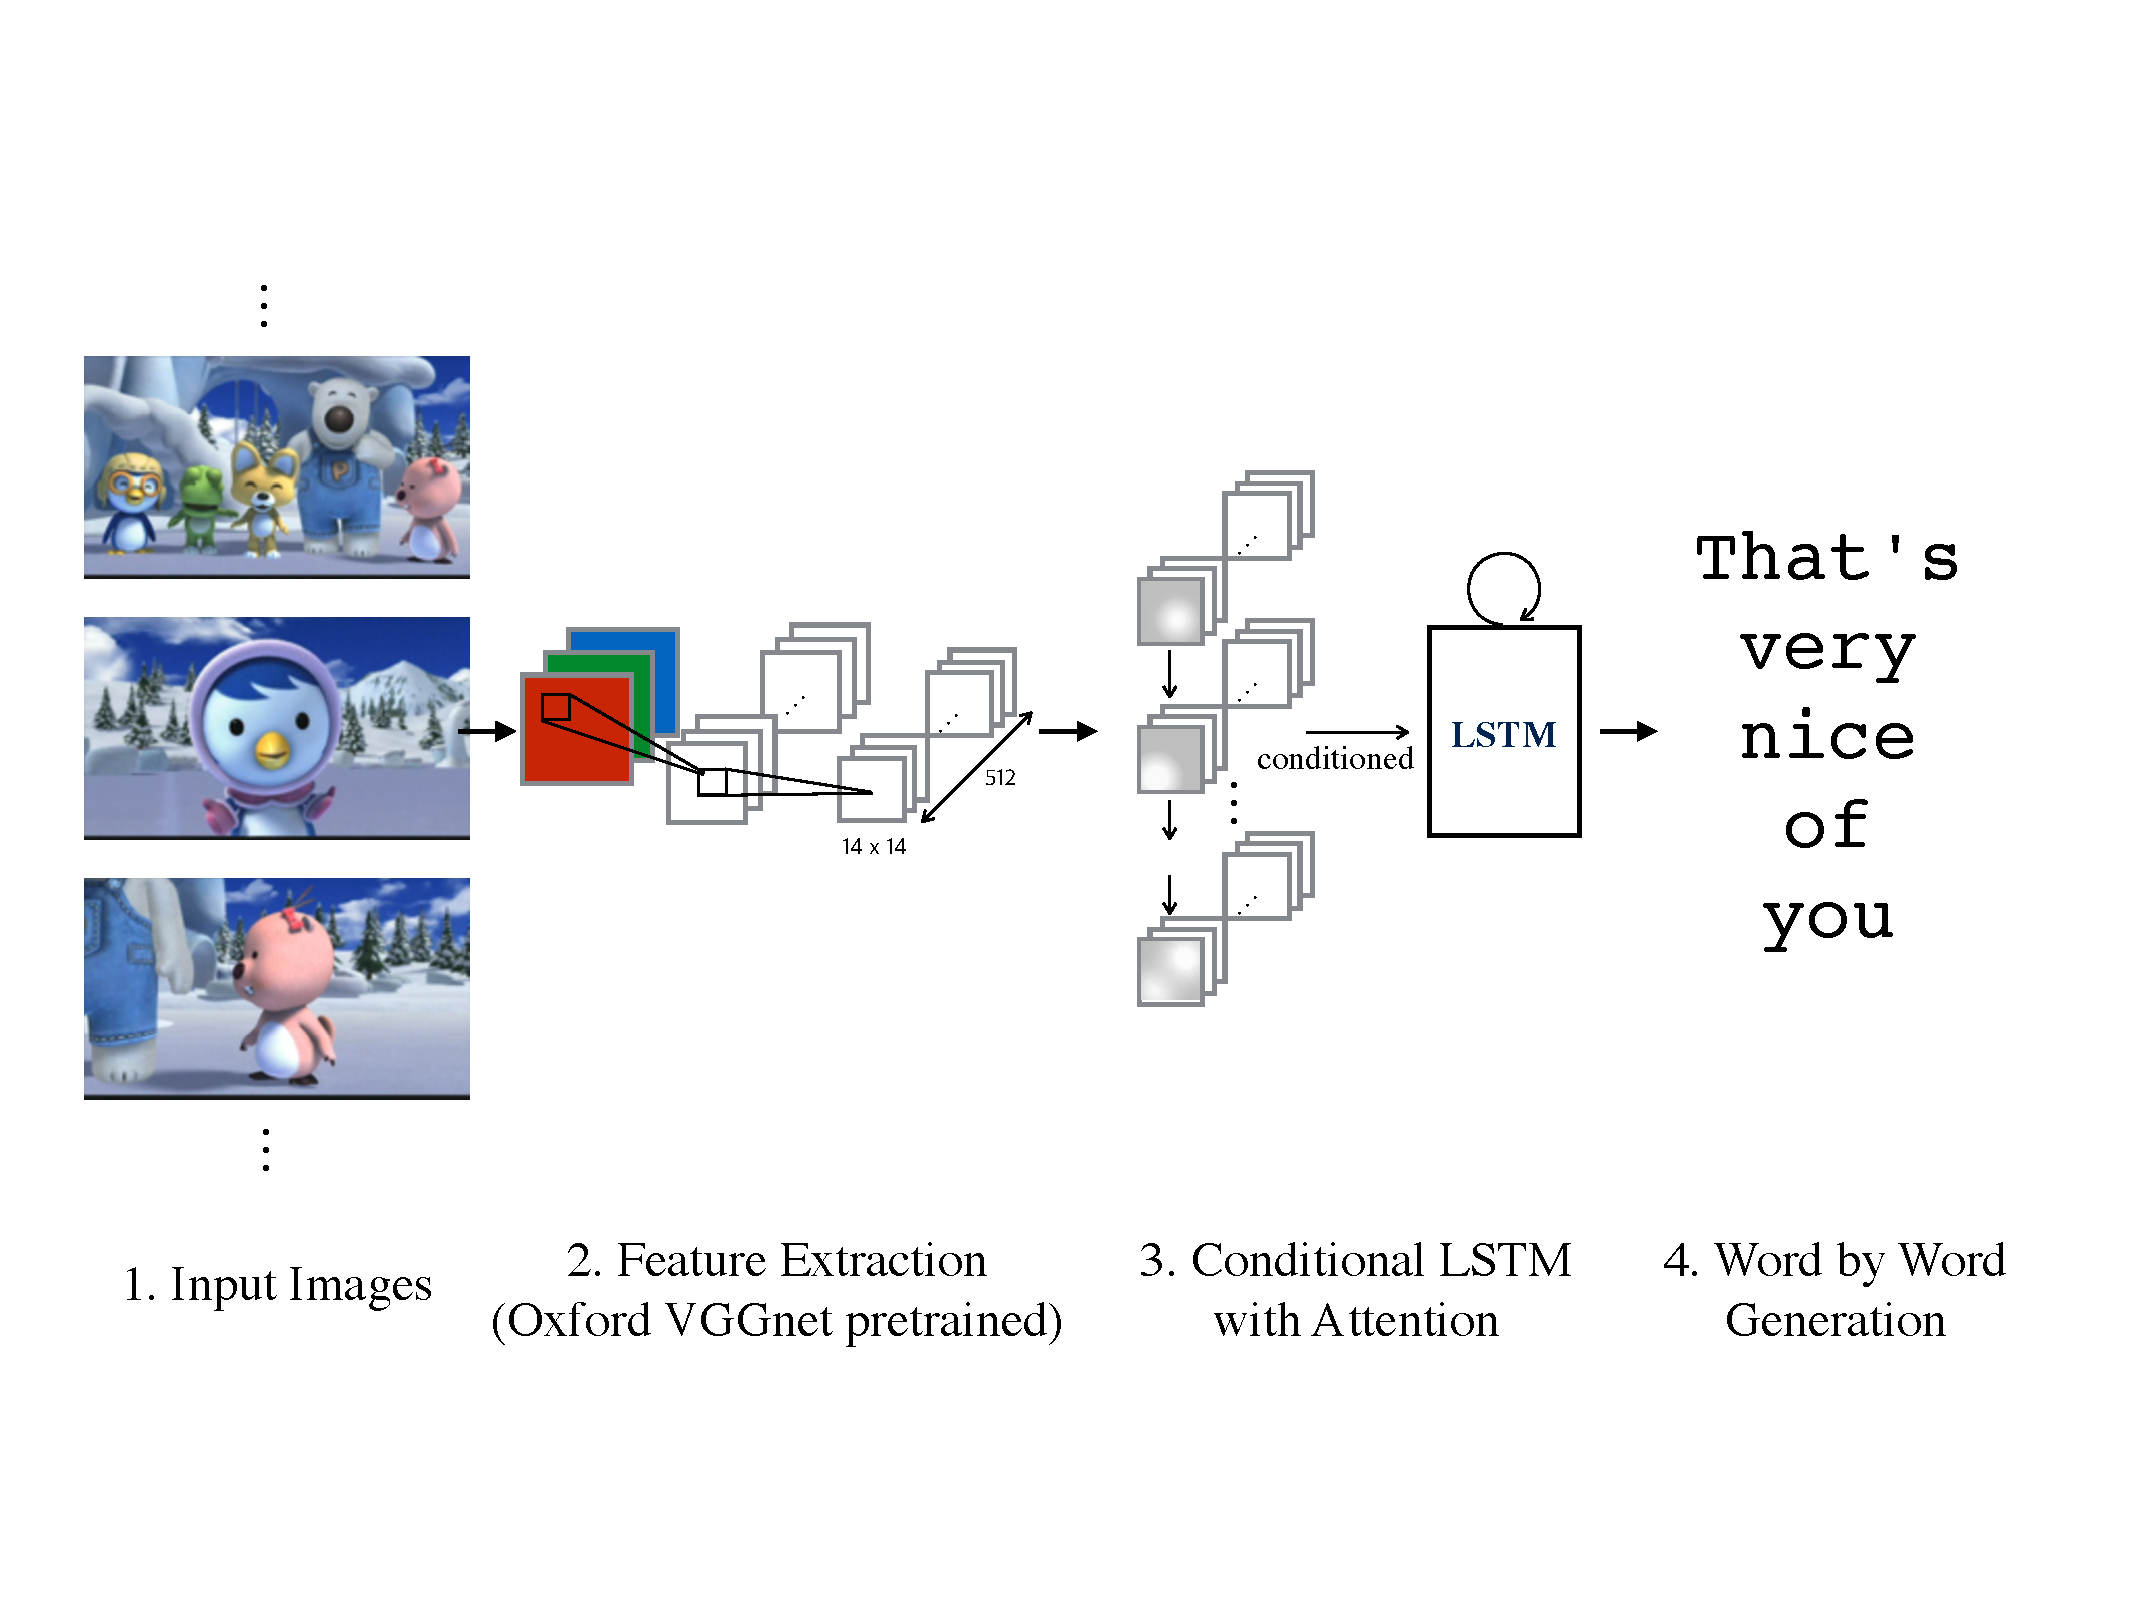
\includegraphics[width=92mm,height=52mm,trim=15mm 40mm 15mm 40mm]{eps/pororo_alstm.pdf}}
  \caption{시선 정보를 활용하는 방법을 도식화. A는 원본 이미지, B는 A를 응시한 서로 다른 13명의 응시 좌표들을 십자가 기호로 표시. C는 응시 좌표들을 가우시안 혼합 모델(Gaussian Mixture Model)로 나타냈을 때의 확률 분포를 등고선 표현. D는 몬테 카를로 방법으로 샘플링할 확률 가중치를 도식적으로 표현.}
  \label{fig:selective}
\end{figure}

하지만 기존 연구는 정적 이미지에 대한 기술적 문장을 생성하도록 학습하기 때문에, 만화 영상과 같이 시간의 흐름에 따라 문맥이 달라질 수 있는 데이터에는 적합하지 않다. 예를 들면 동일한 두 캐릭터가 대화를 나누는 같은 장면도 앞에서 무슨 행동이나 대화를 나누었냐에 따라 문맥이 달라지며 해당 장면에 대한 대사가 달라질 것이다. 따라서 우리는 기술적으로 기존 연구에서 두 가지 요소를 변경하여 문제를 해결하고자 한다. 첫 번째는 LSTM의 메모리 벡터 $\vc_0$와 은닉 벡터 $\vh_0$를 새로운 이미지에 따라 초기화 하지 않고 보존한다. 두 번째는 주의 모델 $\mathbf{f}_{\text{att}}$를 랜덤 파라미터로 초기화하는 대신 한 시간 분량의 비슷하지만 서로 다른 영상을 본 다수 사람들의 시선 분포 정보를 이용하여 파라미터 값을 초기화 함으로써 선택적 학습을 가속화 하고자 한다.  

따라서 본 연구는 입력 이미지들이 시간 축 상에서 문맥적 흐름을 가질 때 한 단어와 이미지의 한 영역의 대응 관계는 문맥에 따라 달라질 수 있다는 가정으로 선행 연구를 확장한다. 이 때 입력 이미지 내 독립 객체들의 상호 작용이 문맥 조건에 따라 달라지고 문장 내의 단어들과의 상호 작용도 더욱 동적으로 일어난다. 

\section{Attentional LSTM}

LSTM 모델은 입력 벡터의 일부가 출력되는 재귀적인 구조를 가진다. $(t-1)$ 시간에서의 출력 벡터 $\vy_{t-1} \in \mathbb{R}^K$의 선형 사영값 $\mE\vy_{\vt-1} \in \mathbb{R}^m$와 은닉 벡터 $\vh_{t-1} \in \mathbb{R}^n$, 그리고 $t$ 시간에서의 문맥 벡터 $\hat{\vz}_t \in \mathbb{R}^D$를 입력하면 $t$ 시간에서의 은닉 벡터 $\vh_t$를 출력한다. 여기에서 $\vy$는 단어를 나타내는 비트 지시 벡터(해당 단어 인덱스가 1이고 나머지는 0인 벡터)이고 $\vh$는 LSTM의 학습 파라미터 벡터, $\hat{\vz}$은 주의 모델 $\mathbf{f}_{\text{att}}$의 출력 값이다. LSTM 모델에서 정규화 방법을 제안한 Zaremba et al.\cite{Zaremba2015}의 방법에 따라 LSTM을 구현하면 다음과 같이 표현할 수 있다.

\begin{equation}
\begin{pmatrix}\mathbf{i_{t}}\\\mathbf{f_{t}}\\\mathbf{o_{t}}\\\mathbf{g_{t}}\end{pmatrix} =
  \begin{pmatrix}\mathrm{\sigma}\\\mathrm{\sigma}\\\mathrm{\sigma}\\\tanh\end{pmatrix}
  \mathbf{T}
  \begin{pmatrix}\mathbf{Ey_{t-1}}\\\mathbf{h_{t-1}}\\\mathbf{\hat{z}_t}\end{pmatrix}
\end{equation}

\begin{equation}
\mathbf{c_t} = \mathbf{f_t} \odot \mathbf{c_{t-1}} + \mathbf{i_t} \odot \mathbf{g_t}\\
\end{equation}
\begin{equation}
\label{eq3}
\mathbf{h_t} = \mathbf{o_t} \odot \tanh(\mathbf{c_t})\\
\end{equation}

$\mE \in \mathbb{R}^{m \times K}$는 단어를 나타내는 비트 지시 벡터를 실수값으로 선형 사영한다.  $\mT \in \mathbb{R}^{(D+m+n) \times n}$는 LSTM의 내부 파라미터 행렬이다. $\mE$와 $\mT$는 연쇄 법칙에 따라 목적 함수에 의해 역전파 알고리즘으로 학습되는 파라미터 행렬이다. 두 개의 초기 값 파라미터, $\mathbf{c}_0$, $\mathbf{h}_0$는 각각 별도의 MLP(Multi-Layer Perceptron)으로 학습하며, 두 MLP는 채널에 대한 $\mathbf{a}$의 평균 값($\in \mathbb{R}^{D}$)을 같은 입력으로 가진다.

수식\ref{eq3}에 따라 $\vh_t$를 구한다면 다음 식을 이용하여 $\vy_t$를 구할 수 있게 된다.

\begin{equation}
p(\vy_t|\vy^{t-1}_1,\sa) \propto \exp{\mL_o(\mE\vy_{t-1} + \mL_{h}\vh_t + \mL_{z}\hat{\vz}_t))}
\end{equation}

여기에서 $\mathbf{L}_{o} \in \mathbb{R}^{K \times m}$, $\mathbf{L}_{h} \in \mathbb{R}^{m \times n}$, $\mathbf{L}_{z} \in \mathbb{R}^{m \times D}$는 모두 목적 함수에 의해 학습되는 파라미터 행렬이다. $\mathbf{a} \in \mathbb{R}^{L \times D}$는 미리 학습된 콘볼루션 네트워크의 반응 값으로 $\mathbf{L}$은 반응 크기(예, $\mathbf{L} = 14 \times 14$), $\mathbf{D}$는 채널 수이다. 

$\mathbf{f_{\text{att}}}$가 반응 벡터 $\va$와 은닉 벡터 $\vh_{t-1}$를 입력으로 하는  MLP일 때, $\mathbf{\hat{z}_t}$는 다음과 같이 정의한다.

\begin{equation}
e_{ti} = \mathbf{f_{\text{att}}}(\mathbf{a_i}, \mathbf{h_{t-1}})
\end{equation}

\begin{equation}
\mathbf{\alpha_{ti}} = \frac{\exp(e_{ti})}{\sum^{L}_{k=1}\exp(e_{tk})}
\end{equation}

\begin{equation}
\mathbf{\hat{z}_t} \sim \text{Multinoulli}_L(\{\alpha_{ti}\})
\end{equation}

문맥 벡터 $\mathbf{\hat{z}_t}$는 역전파 알고리즘으로 학습된 $\mathbf{f_{\text{att}}}$의 결과에 따라 샘플링 된다. 이 때, 목적 함수 $\mathit{L}$을 로그 합 부등식을 이용, marginal log-likelihood $\log p(\mathbf{y}|\mathbf{a})$의 변분 하한으로 정의하고 모델의 파라미터 집합 $W$로 편미분 하면 다음과 같이 정리할 수 있다\cite{Xu2015}. 이 때 $p(\hat{z}|a)$에 대하여 몬테-카를로 샘플링(Monte Carlo sampling) 방법을 사용하여 근사한다.

\begin{equation} 
 \frac{\partial L}{\partial W} \approx \frac{1}{N} \sum_{n=1}^{N} \bigg[ \frac{\partial \log p(\vy \mid \hat{z}, \va)}{\partial W} + 
                                \log p(\vy \mid \hat{z}, \va) \frac{\partial \log p(\hat{z} \mid \va)}{\partial W} \bigg]
\end{equation} 

\section{Story-Aware Attentional LSTM}

만화 영상과 같이 입력 이미지들이 시간 축 상에서 문맥적 흐름을 가질 때 이러한 문맥을 보전하기 위해 이전 기억 상태와 은닉 상태를 유지할 필요가 있다. 따라서, $\mathbf{c_0}$와 $\mathbf{h_0}$를 이전 이미지 $\mathcal{I}_{\text{prev}}$의 마지막 상태 값 $\mathbf{c_T}$와 $\mathbf{h_T}$로 초기화 한다.

$\ff_{\text{att}}$는 콘볼루션 반응 벡터 $a_i$를 은닉 벡터 $\vh_{t-1}$를 통해 샘플링하는 기제를 가진다. 은닉 벡터 $\vh_{t-1}$에 따라 주의 성능에 영향을 미치게 되지만 이는 $\hat{\vz}_{t-1}$에 의존적이므로 만화 영상 데이터에 대한 실험에서 성능을 크게 저하시킬 원인이 된다. 따라서 랜덤 파라미터로 $\ff_{\text{att}}$를 초기화하는 대신 다수 사람들의 시선 분포 정보를 이용하여 파라미터 값을 초기화함으로써 $\ff_{\text{att}}$에 대한 학습을 가속화하고 전체 모델에 대한 효율을 제고 하고자 한다.

관측된 시선 정보에 가우시안 혼합 모델(Gaussian Mixture Model)을 통하여 $\{\tilde{\alpha}_{ti}\}$를 얻은 후, $\vh_{t-1}$는 랜덤 파라미터로 초기화 한 후 $\sa_i$에 대한 $\ff_{\text{att}}$를 학습한다. $\vh_{t-1}$는 $\ff_{\text{att}}$의 상위 층에서 $\sa_i$의 추상 표현과 결합하게 정의하였기 때문에 전이 학습의 효과를 상대적으로 크게 얻을 수 있다\cite{yosinski2014}. 


\begin{figure}
  \centerline{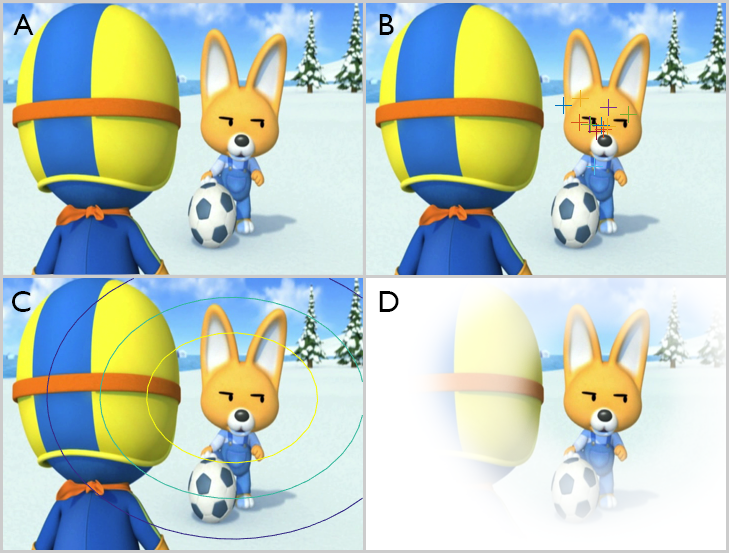
\includegraphics[width=65mm,height=49mm]{eps/sel_fig2.png}}
  \caption{시선 정보를 활용하는 방법을 도식화. A는 원본 이미지, B는 A를 응시한 서로 다른 13명의 응시 좌표들을 십자가 기호로 표시. C는 응시 좌표들을 가우시안 혼합 모델(Gaussian Mixture Model)로 나타냈을 때의 확률 분포를 등고선 표현. D는 몬테 카를로 방법으로 샘플링할 확률 가중치를 도식적으로 표현.}
  \label{fig:selective}
\end{figure}

\section{실험 계획}

콘볼루션 반응 값 $\sa$를 얻기 위해 Oxford VGGnet\cite{Simonyan2014}의 네번째 콘볼루션 층의 max-pooling 바로 전의 반응 값을 사용한다. 반응 크기는 $14 \times 14$, 채널 수는 512 이다. 경험적으로, 일반 이미지에 대한 학습 후에는 학습된 특징 탐지기(feature detectors)들이 충분하기 때문에 추가적인 세밀 조정 학습은 실시하지 않았다. 관찰된 시선 정보에 대한 설명은 그림~\ref{fig:selective}를 참고한다.

\section{토 론}

시간적 문맥과 시각-언어 개념 학습 조건에서는 유연한 모델과 학습 방법을 요구한다 \cite{zhang1994incremental}. 몬테 카를로 방법을 이용한 주의 모델은 한 이미지 내에서 필요한 정보를 능동적으로 탐색하므로 적은 파라미터 수로도 유연한 데이터 적용의 접점을 제공한다.

본 연구에서는 몬테 카를로 방법을 사용하고 있는 주의 모델에서 관찰된 사람의 시선 정보를 이용한다. 다수 사람들의 시선 분포는 시간에 따른 문맥을 고려한 정보이므로 깊은 순환 네트워크 모델의 빠른 수렴을 위한 도움을 준다.

\section{결 론}

기존 연구에서는 LSTM과 MLP에 기반한 주의 모델을 단일한 정보 흐름으로 역전파 알고리즘을 통해 학습할 수 있는 방법을 제안하였다. 그러나 이미지-문장 변환만 고려되어 있어 만화 영상과 같이 시간의 흐름에 따라 문맥이 달라질 수 있는 데이터에는 적합하지 않았다. 본 연구에서는 메타 정보인 사람의 시선 분포 정보를 이용하여 시간에 따른 문맥 정보를 고려할 때 발생할 수 있는 계산 비용 문제를 풀고자 하였다.  

\section{감사의 글}
이 논문은 2015년도 정부(미래창조과학부)의 재원으로 한국연구재단의 지원(NRF-2010-0017734-Videome)과 정보통신기술진흥센터의 지원(R0126-15-1072-SW스타랩, 10035348-mLife, 10044009-HRI.MESSI)을 받아 수행된 연구임.

\bibliographystyle{ieeetr}
\bibliography{KidsVideo-selective}

\end{document}
